\section{Experimental Evaluation}
\label{sec:experiments}

We evaluate the proposed transition certificate synthesis methods on two benchmark systems to demonstrate their effectiveness in formal LTL verification and their computational advantages. We compare against three baselines: the state-triplet method~\cite{wongpiromsarn2015automata}, closure certificates~\cite{murali2024closure}, and neural closure certificates~\cite{nadali2024neural}. For the first benchmark, the Kuramoto Oscillator model (covering both 1D and 2D scenarios), we verify the system against specified LTL properties. For the second benchmark, the two-room temperature model, we demonstrate the versatility of our approach by synthesizing transition certificates to satisfy complex LTL requirements and highlight their complementary advantages in handling diverse temporal specifications. All experiments are conducted on Ubuntu 22.04.3 LTS (Intel i7-9750H, 8 GB RAM). During candidate generation, Z3 addresses the constrained optimization for polynomial templates, whereas neural network templates are trained using the Adam optimizer (learning rate 0.001, 1000 iterations) to minimize the loss function. For formal verification, we employ dReal (precision 0.0001) to handle the transcendental $\sin$ functions in the Kuramoto Oscillator model, while Z3 is utilized for the temperature model. 

\subsection{Kuramoto Oscillator}
\subsubsection{One-Dimensional System}
% 系统介绍
The first benchmark is a Kuramoto oscillator system, formally defined as $\mathfrak{S} = (\mathcal{X}, \mathcal{X}_0, f)$ with dynamics adapted from~\cite{anand2022small}. The system operates within the state space $\mathcal{X} = [0, 2\pi]$, starting from an initial region $\mathcal{X}_0 = [\frac{4\pi}{9}, \frac{5\pi}{9}]$. To evaluate LTL verification, we specify an unsafe region $\mathcal{X}_u = [\frac{7\pi}{9}, \frac{8\pi}{9}]$ within the temporal properties. The discrete-time transition function $f$ is given by:
\begin{align}
f(x) = x + t_s\Omega + t_s K \sin(-x) - 0.532 x^2 + 1.69,
\end{align}
where $x$ represents the oscillator phase. The system parameters are set as follows: sampling time $t_s = 0.1$, natural frequency $\Omega = 0.01$, and coupling strength $K = 0.0006$.



% 如何将安全性验证转化为LTL验证
We consider the LTL specification $\phi = \mathbf{G}\neg a$ over the atomic proposition set $AP = \{a\}$, with the labeling function defined as $\mathfrak{L}(x) = \{a\}$ for $x \in \mathcal{X}_u$ and $\mathfrak{L}(x) = \emptyset$ otherwise. The negated specification, $\neg \phi = \mathbf{F} a$, is characterized by the NBA illustrated in Figure~\ref{pic-tbnba1}. This automaton incorporates accepting transitions $(q_0, \emptyset, q_0)$ and $(q_0, \{a\}, q_0)$ originating from the initial state $q_0 \in Acc^{\text{start}}$.

\begin{figure}[h]
  \centering
  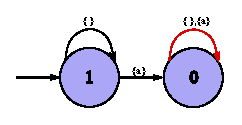
\includegraphics[width=0.3\textwidth]{pic/tbnba1.eps}
  \caption{NBA representing the negated specification $\mathbf{F} a$. Accepting transitions (highlighted in red) are depicted as self-loops at state $q_0$.}
  \label{pic-tbnba1}
\end{figure}

% 多项式模板方法
Based on the definition of transition safety certificates, we implement a polynomial-based CEGIS framework to synthesize certificates that guarantee the satisfaction of the specified LTL property. The polynomial template is structured as follows:
\[
B_0(x, q; \mathbf{c}) = \sum_{i=0}^{4} c_i x^i + \sum_{j=1}^{3} c_{4+j} q^j + c_8 xq.
\]
The synthesis process begins by collecting 30 samples from region $D_0$, 600 from $D_u$, and 1200 from $D_{\mathcal{X}}$. The candidate generation phase is formulated as a constraint satisfaction problem and solved using the Z3 solver. Given that the system dynamics involve the transcendental $\sin$ function, which lies beyond the decision procedures of Z3, we employ the dReal solver during the verification phase to identify counterexamples. The complete CEGIS loop converges in 1.76 seconds, successfully yielding a valid transition certificate:
\[
B_0(x, q) = -1 + 2q^2 - \frac{7}{16}xq.
\]

% 神经模板方法
In addition to polynomial templates, we synthesize a neural transition certificate $B_0(x, q; \theta)$ using the CEGIS framework. The certificate is parameterized by a feedforward neural network with a 2-10-1 architecture, featuring two input nodes for the pair $(x, q)$, a hidden layer of 10 neurons with ReLU activation, and a single linear output. The training process is initialized with a dataset of 250 samples (40 from $D_0$, 70 from $D_u$, and 140 from $D_{\mathcal{X}}$). During each iteration, the dReal solver is employed to identify any points violating the certificate conditions. These identified counterexamples are then incorporated into the training set to progressively refine the candidate certificate. The complete CEGIS loop converges in 6.81 seconds. The valid certificates obtained during the process are provided in the appendix.

For comparison, the state-triplet method~\cite{wongpiromsarn2015automata} synthesizes a barrier certificate for the relevant simple path in 0.10 seconds under a degree-4 polynomial template. The certificate $B(x)=-4.5x^2+2x^3$ blocks the accepting state via the state-triplet barrier conditions; one accepting edge is discharged trivially because its label region is empty.

\subsubsection{Two-Dimensional System}

The benchmark is further extended to a two-dimensional scenario with state space $\mathcal{X} = [0, \frac{8\pi}{9}]^2$ and initial region $\mathcal{X}_0 = [0, \frac{\pi}{9}]^2$. In this case, the unsafe region $\mathcal{X}_u$ is defined as the boundary corridors of the state space:
\begin{equation}
\mathcal{X}_u = \left([0, \tfrac{8\pi}{9}] \times [\tfrac{5\pi}{6}, \tfrac{8\pi}{9}]\right) \cup \left([\tfrac{5\pi}{6}, \tfrac{8\pi}{9}] \times [0, \tfrac{8\pi}{9}]\right).
\end{equation}
The coupled system dynamics $f$ are governed by:
\begin{equation}
f(x_1, x_2) =
\begin{bmatrix} x_1 \\ x_2 \end{bmatrix}
+ t_s
\begin{bmatrix} \Omega + 1.69 \\ \Omega + 1.69 \end{bmatrix}
+ K t_s
\begin{bmatrix} \sin(x_2 - x_1) \\ \sin(x_1 - x_2) \end{bmatrix}
- 0.532 t_s
\begin{bmatrix} x_1^2 \\ x_2^2 \end{bmatrix}.
\end{equation}
To maintain consistency with the 1D analysis, we define the labeling function such that $\mathfrak{L}(x_1, x_2) = \{a\}$ if $(x_1, x_2) \in \mathcal{X}_u$ and $\emptyset$ otherwise. The verification is performed against the same LTL specification $\phi = \mathbf{G}\neg a$ using the NBA illustrated in Figure~\ref{pic-tbnba1}.


For the two-dimensional system, we first employ a polynomial template $B_0(x_1, x_2, q; \mathbf{c})$. The synthesis process utilizes a dataset of 30 samples from $D_0$, 729 from $D_u$, and 1,458 from $D_{\mathcal{X}}$. Within 1.72 seconds, the CEGIS loop yields a valid transition certificate:
\begin{equation}
B_0(x_1, x_2, q) = -1 + \tfrac{1}{8}x_1 x_2 + \tfrac{3}{2}q^2 - \tfrac{3}{32}q x_1^2 - \tfrac{153}{512}x_2 q.
\end{equation}
Furthermore, we implement a neural network template with a 3-15-1 architecture, featuring three input nodes for the tuple $(x_1, x_2, q)$ and a hidden layer of 15 neurons with ReLU activation. To demonstrate the efficiency of our framework, we initialize the training with a set of points: 40 from $D_0$, 90 from $D_u$, and 180 from $D_{\mathcal{X}}$. The CEGIS loop converges in 110.95 seconds, successfully producing a valid neural certificate in appendix.

For comparison, the state-triplet method~\cite{wongpiromsarn2015automata} synthesizes a barrier certificate for the relevant simple path in 1.13 seconds under a degree-2 polynomial template, yielding $B(x_1,x_2)=-x_1-x_2-3.125x_1x_2+2x_1^2+2x_2^2$.

\subsection{Two-Room Temperature}

The second benchmark focuses on the formal verification of an interconnected temperature control system, denoted by $\mathfrak{S} = (\mathcal{X}, \mathcal{X}_0, f)$, with its dynamical model adapted from~\cite{anand2024compositional}. The system operates within a state space $\mathcal{X} = [20, 34]^2$, originating from the initial configuration $\mathcal{X}_0 = [21, 24]^2$. The underlying LTL specification pertains to the target region $\mathcal{X}_{VF} = [20, 26]^2$. Specifically, the evolution of the system state is governed by the following discrete-time dynamics $f$:
\begin{equation}
f(x_1, x_2) = 
\begin{bmatrix} 1 - 2\alpha - \theta - \mu u(x_1) & \alpha \\ \alpha & 1 - 2\alpha - \theta - \mu u(x_2) \end{bmatrix}
\begin{bmatrix} x_1 \\ x_2 \end{bmatrix}
+ \mu T_h
\begin{bmatrix} u(x_1) \\ u(x_2) \end{bmatrix}
+ \theta
\begin{bmatrix} T_e \\ T_e \end{bmatrix},
\end{equation}
where the constant parameters are assigned as $\alpha = 0.004$, $\theta = 0.01$, $\mu = 0.15$, $T_h = 40$, and $T_e = 0$. The state-dependent control term is defined as $u(x_i) = 0.59 - 0.011 x_i$ for $i \in \{1, 2\}$.



Consider the set of atomic propositions $AP = \{a, b\}$, where the labeling function is defined as $\mathfrak{L}(x_1, x_2) = \{a\}$ for $(x_1, x_2) \in \mathcal{X}_0$, and $b \in \mathfrak{L}(x_1, x_2)$ for $(x_1, x_2) \in \mathcal{X}_{VF}$. The system is required to satisfy the LTL specification $\phi = a \Rightarrow \mathbf{FG}\neg b$. The corresponding NBA, which captures the negation of the specification (i.e., $\neg \phi = a \land \mathbf{GF} b$), is illustrated in Figure~\ref{pic-tbnba2}. Since $q_1$ is the only accepting-transition start state and the initial region $\mathcal{X}_0 = [21,24]^2$ is entirely labeled $\{a\}$ by $\mathfrak{L}$, the automaton transitions to $q_1$ at the very first step from any initial product state. This makes $q_1$ immediately reachable, so a transition safety certificate for $q_1$ cannot be found. We therefore apply a transition persistence certificate to bound the number of times the accepting transitions from $q_1$ can fire.


\begin{figure}[h]
  \centering
  
\includegraphics[width=0.3\textwidth]{pic/tbnba2.eps}
  \caption{NBA for $a \land \mathbf{GF} b$ (negation of $a \Rightarrow \mathbf{FG}\neg b$). Accepting transitions (red) are $(q_1, \{b\}, q_1)$ and $(q_1, \{a,b\}, q_1)$.}
  \label{pic-tbnba2}
\end{figure}

Consider the transition persistence certificate template (see Appendix~\ref{appendix-experiment}). We collect 16 samples for $D_0$ and 196 for $D_{\mathcal{X}}$. We obtain a valid transition persistence certificate $$B_{1,1}(x_1, x_2) = 27 I_{[20,26]^2}(x_1, x_2) - x_1 I_{[20,26]^2}(x_1, x_2)$$ and $\epsilon = 0.25$ in 2.68 seconds.

We apply the neural CEGIS to synthesize $B_{1,1}(x_1, x_2)$ for $Acc^{1,1}$, using a neural network template of architecture 2-3-1 (2 inputs for $(x_1, x_2)$, 3 hidden neurons with squared activation, 1 output). We collect 100 samples for $D_{\mathcal{X}}$ and 16 samples for $D_0$. The entire CEGIS loop terminates in 1461.91 seconds and the valid certificates obtained are provided in the appendix.

In contrast, the state-triplet method~\cite{wongpiromsarn2015automata} times out on this benchmark. The accepting path cannot be blocked by a barrier certificate within the time limit, because the initial region is entirely contained within the target region $\mathcal{X}_{VF}$, making the accepting automaton state reachable and the state-triplet's path-blocking obligation too conservative.

\subsection{Comparison}
We primarily compare our approach with the state-triplet method~\cite{wongpiromsarn2015automata} and closure certificates~\cite{murali2024closure}. The state-triplet method is a foundational automata-theoretic approach that constructs barrier certificates to block all simple paths from initial states to accepting states in the automaton, requiring enumeration of state triplets along these paths. Closure certificates were specifically developed to provide more general verification conditions than the state-triplet method, and neural closure certificates~\cite{nadali2024neural} extend this idea with neural network templates. The Two-Room Temperature benchmark concretely illustrates the advantage over the state-triplet method. The NBA contains an accepting transition from $q_1$ to $q_1$ labeled by $\{b\}$ and $\{a,b\}$, and because the labeling function maps the entire initial region $\mathcal{X}_0=[21,24]^2$ to $\{a\}$, the automaton state $q_1$ is immediately reachable upon entering the product system. Consequently, the state-triplet approach, which requires blocking all paths to accepting states via barrier certificates, is structurally inapplicable here since $q_1$ cannot be made unreachable, leading to a timeout. Our transition persistence certificate $B_{1,1}$ resolves this by bounding the number of times the accepting transition can fire, without requiring $q_1$ to be unreachable. The core idea of closure certificates lies in characterizing an over-approximation of the transition closure, so closure certificates for LTL verification are defined over $\mathcal{X} \times \mathcal{X} \times Q \times Q$. In contrast, our method employs transition safety certificates to directly filter out unreachable automaton states or uses transition persistence certificates to prove that the accepting transitions occur finitely often, with transition safety certificates defined over $\mathcal{X} \times Q$ and transition persistence certificates defined over $\mathcal{X}$ alone. This reduces the effective certificate domain from the closure certificate's $\mathcal{X} \times \mathcal{X} \times Q \times Q$ to at most $\mathcal{X} \times Q$, and improves synthesis efficiency. For neural templates, we adopt the CEGIS framework, whereas the neural closure certificate approach relies on sampling and posteriori verification: after sampling the state space with a given density $\epsilon$ and safety margin $\eta$, the method trains until the loss converges to zero and then performs a posteriori verification to determine whether the synthesized certificate is valid.

We conduct two groups of comparisons: (1) polynomial-template CEGIS versus the state-triplet method and closure certificates, and (2) neural-template CEGIS versus neural closure certificates. The detailed experimental configurations are provided in Appendix~\ref{appendix-experiment}. Table~\ref{tab:results-poly} and Table~\ref{tab:results-neural} report only locally reproduced, formally verified results under a five-hour timeout. For the CC and NCC baselines, the implementations follow the original synthesis-and-verification schemes; previous guarded-transition or interval-overapproximation variants are not counted in these tables. ``Timeout'' means that no formally verified certificate was produced within the timeout. The original closure-certificate paper reports successful CC synthesis on these benchmarks, but until the corresponding faithful local rerun produces a verified certificate, the reproduced entry is recorded as Timeout.

The comparison separates proof soundness from search success. The theorems in Section~\ref{sec:method} state that a certificate satisfying the displayed inequalities proves the corresponding LTL property. The experiments evaluate whether the chosen polynomial or neural template, solver configuration, and finite synthesis budget can find such certificates on the benchmark instances. Thus a timeout or an unsuccessful bounded diagnostic is evidence about the tested search procedure and template capacity, not a counterexample to the transition-certificate proof rule and not evidence that a baseline paper is incorrect.

\begin{table}[t]
\centering
\caption{Synthesis time comparison for polynomial-template methods (seconds)}
\label{tab:results-poly}
\begin{tabular}{lccc}
\hline
\textbf{Benchmark} & \textbf{Transition Certificates} & \textbf{State Triplet} & \textbf{Closure Certificate} \\
\hline
Kuramoto 1D & 1.76 & 0.10 & Timeout \\
Kuramoto 2D & 1.72 & 1.13 & Timeout \\
Two-Room Temperature & 2.68 & Timeout & Timeout \\
\hline
\end{tabular}
\end{table}
\begin{table}[t]
\centering
\caption{Synthesis time comparison (seconds)}
\label{tab:results-neural}
\begin{tabular}{lcc}
\hline
\textbf{Benchmark} & \textbf{Transition Certificates} & \textbf{Neural Closure Certificate} \\
\hline
Kuramoto 1D & 6.81 & Timeout \\
Kuramoto 2D & 110.95 & Timeout \\
Two-Room Temperature & 1461.91 & Timeout \\
\hline
\end{tabular}
\end{table}
